\chapter{A Crash Course in PL Topology}\label{appendix:pl-topology}
\epigraph{What is the big-picture idea of Linear Algebra? Reduce
  infinite spaces to finite descriptions. That is it---\emph{this} is
  the meaning of a basis!}{---Weiqing Gu}
\def\figdir{figures/appendix/}

For our purposes today, we can think of Piecewise-Linear Topology as
``the business of trying to study continuous topological objects by
approximating them with linear (more accurately, affine) structures.''
Because such structures can be given finite descriptions, there is a
sense in which this will bring a more ``discrete'' flavor to our
topological objects. Of particular importance will be the concept of a
\emph{simplicial complex}, what it means for one to be \emph{locally
  finite}, and how we can use this to build up our understanding of
knots. We'll begin by discussing some vocabulary. % The exposition here
% follows that in \cite{Sakai2013} fairly closely; see there for more
% details.\footnote{For our personal tastes, we found \cite{Sakai2013} a
%   bit difficult to read, especially given the sparsity of diagrams /
%   visuals. However, we did find it to be quite thorough.}

\section{Affine Sets}
Really we'll only be interested in convex sets for today. But to
define them, we need the concept of \emph{affine independence}, so it
seemed reasonable to do a brief primer on \emph{affine} topics while
we're at it.

Everything in the below should be general over any Banach space with
field $\RR$, but for today, we'll only consider $\RR^n$.% Note, in the
% below, we'll actually often write $\RR^m$ since we'll use $n$ to refer
% to an $n$-cell.
\begin{definition}[Affine Set]
  Let $F \subseteq \RR^n$. Then $F$ is called a \emph{affine set}
  (also sometimes called a \emph{flat}, but we won't use that here) if
  for all $x,y \in F$ and $t \in \RR$, we have
  \[
    \bk{1-t} x + ty \in F.
  \]
  Geometrically, ``every line through two points in $F$ is itself a
  subset $F$.''
\end{definition}
Note, this is essentially just a linear subspace that we allow to be
shifted so as to not include the $0$ vector. For instance:
\begin{figure}[H]
  \centering
  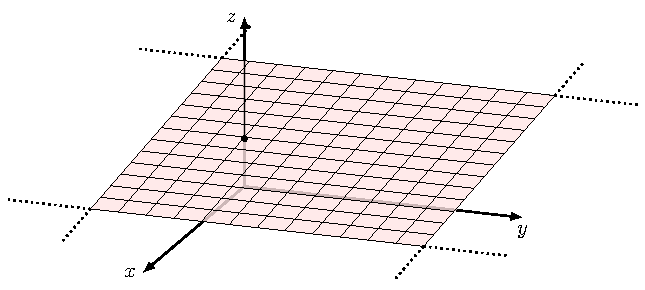
\includegraphics{figures/wild/affine-set.pdf}
  \caption[An affine set]{An affine set. The black circle indicates a
    point of intersection.}
  \label{fig:affine-set}
\end{figure}
\noindent is an affine set. This is encoded in the following
proposition.
\begin{proposition}\label{prop:affine-to-linear}
  Let $F \subseteq \RR^n$ be an affine set. Then for arbitrary $x \in
  F$, $F - x = \set{v - x \MID v \in F}$ is a linear subspace of
  $\RR^n$.
\end{proposition}
As an example, imagine shifting the plane in \cref{fig:affine-set}
down to the origin.

Just as we have a notion linear independence for vector spaces, we
have affine independence for affine sets.
\begin{definition}[Affine Independence]
  Let $\set{v_i}_{i=1}^n \subseteq \RR^n$. Then we say $\set{v_i}$
  are \emph{affinely-independent} iff % for all $\set{t_i}_{i=1}^n \in
  % \RR$, if
  % \[
  %   \sum_{i =1}^n  t_i v_i = 0 \qquad\qquad\text{and}\qquad\qquad
  %   \sum_{i=1}^n t_i = 0,
  % \]
  % then for all $i = 1, \ldots, n$, we have $t_i = 0$. This is
  % equivalent to requiring that
  for any $j = 1, \ldots, n$, the set
  \[
    \mc B_j = \set{v_i - v_j \MID % i= 1, \ldots, n \text{ where }
      i \neq j}
  \]
  is linearly independent.
\end{definition}
Note again, by \cref{prop:affine-to-linear}, this is just saying we
have a shifted linear subspace. We now define an analog to the
\emph{span} of a linearly independent set.
\begin{definition}[Affine Hull]
  Let $A \subset \RR^n$ be arbitrary. Then the \emph{affine hull} of
  $A$, denoted $\aff(A)$, is given by
  \[
    \aff(A) = \set{\sum_{i=1}^k t_i x_i \MID k \in \NN^{> 0},\
      \text{each}\ t_i \in \RR,\ x_i \in A, \text{ and } \sum_{i=1}^k
      t_i = 1% \ \text{and each}\ t_i \in \RR \text{ and }
      % x_i \in A
    }. \qedhere
  \]
\end{definition}
Note, we require $k > 0$ so that we don't accidentally pick up the
$0$ vector. One can use \cref{prop:affine-to-linear} to verify the
following:
\begin{proposition}
  Let $X \subseteq \RR^n$, and let $v \in F$. Then $\aff(X) - v =
  \vspan{X-v}$.
\end{proposition}
This formalizes our intuition that the affine hull is essentially a
shifted version of linear span. Finally, we introduce the analog to
linear transformations, namely \emph{affine maps}. These are
essentially just linear transformations followed by shifts; we'll use
them later to define PL maps.
\begin{definition}[Affine Map]
  Let $n,m \in \NN$, and let $A \subseteq\RR^n$, $B \subseteq \RR^m$
  be affine sets.\footnote{We make no assumptions about the relative
    sizes of $n,m$.} Then $f : A \to B$ is said to be affine iff for
  all $x,y \in A$ and all $t \in \RR$, we have
  \[
    f\pn{[1-t]x + ty} = [1-t] f(x) + tf(y). \qedhere
  \]
\end{definition}
Note, it was important to require both $A$ and $B$ to be affine in
order to guarantee we don't escape the domain / codomain in the
equation above. Again, we can reduce this to more familiar terms with
the following proposition.\footnote{This basically says ``affine maps
  can be thought of as shifting the affine set to the origin, applying
  a linear transformation, and then shifting it somewhere else.''}
\begin{proposition}
  Let $A \subseteq \RR^n$, $B \subseteq \RR^m$ be affine sets, and let
  $f : A \to B$. Then $f$ is affine iff for all $v_0 \in A$, the
  function $ f_{v_0} : \np{F - x_0} \to \np{B - f(x_0)}$ defined by
  \[
    f^{v_0}(v) = f(v + v_0) - f(v_0)
  \]
  is linear.
\end{proposition}
In interpreting the above, it might be helpful to note that by
\cref{prop:affine-to-linear}, $F - x_0$, $B - f(x_0)$ are linear
subspaces of $\RR^n, \RR^m$ respectively. Also note that on the
right-hand-side, we need the $+v_0$ in the $f(v + v_0)$ to ensure that
we are feeding $f$ something that really is in its domain.

Alright! This gives us everything we need to discuss convex sets and
simplicial complexes.

\section{Convex Sets, Simplices, \& Cells}
Convex sets are (more or less) restricted versions of affine sets.
Recall, in defining affine sets, we were essentially requiring that
any point $p$ on a line passing through points $x,y$ of our space $A$
had to also be an element of $A$. For convex sets we'll do something
similar, only instead of a \emph{line} passing through $x,y$, we look
at \emph{line segments} with endpoints $x,y$. This is encoded in the
following definition.
\begin{definition}[Convex Sets]
  Let $X \subseteq \RR^n$. Then we say $X$ is \emph{convex} iff for
  all $x,y \in X$ and $t \in [0,1]$, we have
  \[
    [1-t]x + ty \in X. \qedhere
  \]
\end{definition}
Note, affine sets are trivially convex. Just as we defined the affine
hull to mimic span for affine sets, we'll define the convex hull to
mimic span for convex sets.
\begin{definition}[Convex Hull]
  Let $A \subseteq \RR^n$. Then the \emph{convex hull} of $A$ is given
  by \footnotesize
  \[
    \ip{A} = \set{\sum_{i=1}^k t_i x_i \MID t_1 + \cdots + t_k = 1,\
      \text{and}\ \np{\text{for all}\ i = 1, \ldots, k,\ t_i \geq 0\
        \text{and}\ x_i \in A}
    }. \qedhere
  \]
\end{definition}

\section{Simplices \& Cells and their Complexes}
Note, in this section, we mostly follow the exposition in J.\ L.\
Bryant's \emph{Piecewise Linear Topology}, which we found the most
readable of the sources we referenced.\footnote{Can be found here:
  \url{https://www.maths.ed.ac.uk/~v1ranick/papers/pltop.pdf}}

\begin{definition}[Simplex]
  Let $\set{v_i}_{i=1}^n$ be affinely independent in $\RR^m$. Then the
  convex hull $\sigma = \ip{\set{v_i}_{i=1}^n}$ is called an $n-1$
  \emph{simplex}.
\end{definition}
\begin{definition}[Face]
  Let $\sigma = \ip{v_i}_{i=1}^n$. Then for all subsets $J \subseteq
  \set{1, \ldots, n}$, we call $\tau = \ip{v_j}_{j\in J}$ a
  \emph{face} of $\sigma$. We will often denote this by $\tau
  <\sigma$.
\end{definition}
\begin{definition}[Convex Linear Cell]
  $A \subseteq \RR^m$ is called a \emph{convex linear cell} iff
  there exist $v_1, \ldots, v_k$ (\emph{not} necessarily affinely
  independent) such that
  \[
    A = \ip[]{\set{v_i}_{i=1}^k}.
  \]
  If $n$ is the size of a maximal affinely independent subset of
  $A$, we say $A$ is a \emph{convex linear $n-1$-cell}.
\end{definition}
\begin{remark}
  Note, every convex linear $n$-cell $A$ can be written as
  \[
    A = \bigcup_{i=1}^{\ell} \sigma_i
  \]
  where the $\sigma_i$ are $n$-simplices without any ``gaps''
  between them.
\end{remark}



\begin{definition}[Simplicial Complex]
  Let $K = \set{\sigma_i}$, where the $\sigma_i$ are all $k$-simplices
  in $\RR^n$. Then we call $K$ a \emph{simplicial complex} iff
  \begin{enumerate}[label=(\arabic*)]
    \item (\textbf{Closure under faces}): For all $\sigma \in K$, for
      all faces $\tau \subseteq \sigma$, we have $\tau \in K$ as well.
    \item (\textbf{Intersection only along faces}): For all $\sigma,
      \tau \in K$, if $\sigma \cap \tau \neq \varnothing$, then
      $\sigma \cap \tau$ is a face of both $\sigma$ and $\tau$.
      \qedhere
  \end{enumerate}
\end{definition}
As an example, the following is a simplicial complex defined by taking
the standard tetrahedron and including each of its faces:
\begin{figure}[H]
  \centering
  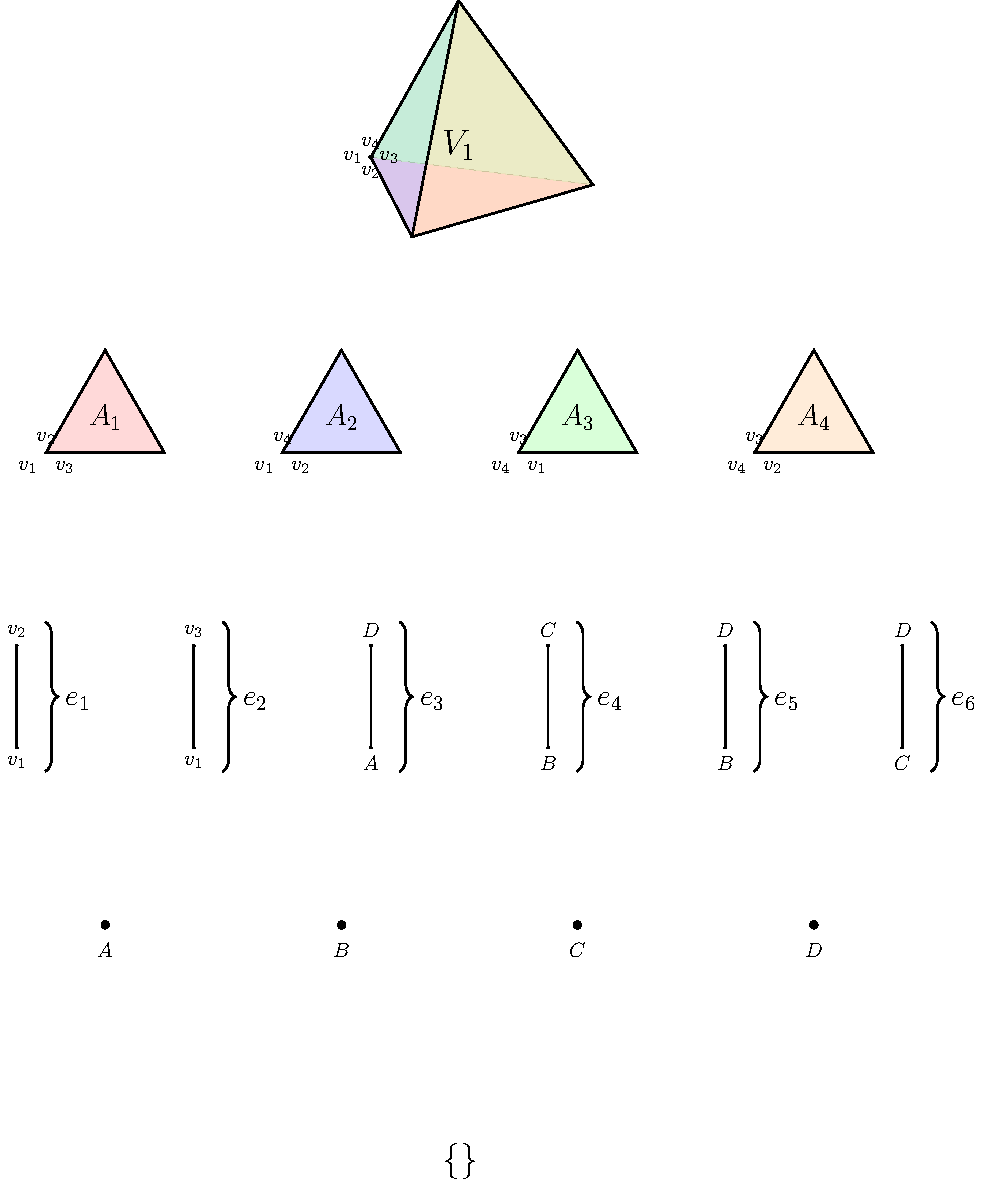
\includegraphics[scale=.5]{\figdir/simplicial-complex.pdf}
  \caption{Example simplicial complex}
\end{figure}
In particular, $K = \set{V_1, A_1, A_2, A_3, A_4, e_1, e_2, e_3, e_4,
  e_5, e_6, A, B, C, D, \set{}}$.

The following proposed ``complex'' fails condition (2):
\begin{figure}[H]
  \centering
  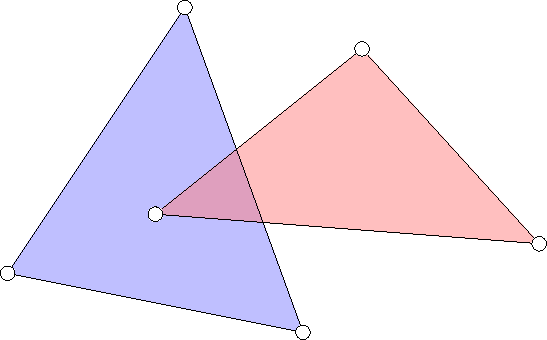
\includegraphics{\figdir/simplex-collision.pdf}
  \caption{An example of a collection $K$ that fails condition (2).}
\end{figure}
We can perform a resolution by subdividing faces until the condition
is regained:
\begin{figure}[H]
  \centering
  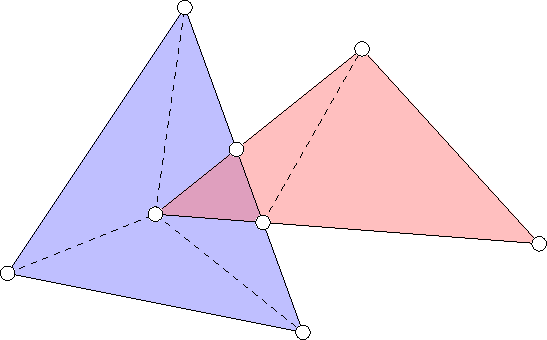
\includegraphics{\figdir/simplex-collision-resolution-1.pdf}
  \caption{Subdividing to resolve the problem.}
\end{figure}
\begin{figure}[H]
  \centering
  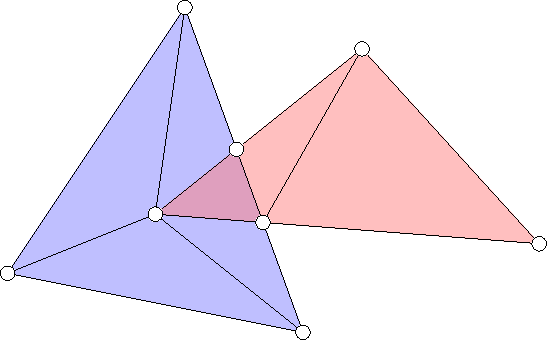
\includegraphics{\figdir/simplex-collision-resolution-2.pdf}
  \caption{The new complex.}
\end{figure}
\begin{definition}[Polyhedron]
  Let $K = \set{\sigma_i}$ be a simplicial complex. Then the
  \emph{polyhedron} of $K$ (also called the \emph{underlying space} of
  $K$), denoted $\abs{K}$, is defined by
  \[
    \abs{K} = \bigcup_{\sigma \in K} \sigma. \qedhere
  \]
\end{definition}
We think of $\abs{K}$ as being endowed with the \emph{weak} topology,
which (given some niceness constraints) coincides with the subspace
topology.
\begin{definition}[Weak topology]
  Let $K$ be a simplicial complex. Define the \emph{weak topology} on
  $\abs{K}$ as follows:
  \begin{leftbar}
    Let $U \subseteq \abs{K}$ be arbitrary. Then we say $U$ is open
    iff for all $\sigma_i\in K$, $U \cap \sigma_i$ is open in
    $\sigma_i$. \qedhere
  \end{leftbar}
\end{definition}
The appropriate niceness constraint is provided by \emph{local
  finiteness}. This is defined slightly differently in different
texts.
\begin{definition}[Locally Finiteness]\label{def:locally-finite}
  Let $K = \set{\sigma_i}$ be a simplicial complex. Then we say $K$ is
  \emph{locally finite} if for all $0$-simplices $v \in K$, there
  exists $\varepsilon > 0$ such that there exists only finitely-many
  $\sigma_i$ for which
  \[
    \sigma_i \cap B_\varepsilon(v) = \varnothing.
  \]
\end{definition}
Note, other sources might define local finiteness in a different
manner. Namely,
\begin{definition}[Local Finiteness (Alt.)]\label{def:locally-finite-bad}
  Let $K$ be a simplicial complex. Then we say $K$ is \emph{locally
    finite} if for all $0$-simplices $v \in K$, there exists only
  finitely-many $\sigma_i$ such that $v$ is a vertex of $\sigma_i$.
\end{definition}
As far as we can tell, these conditions are not equivalent, but we
could be missing something here. For instance, under
\cref{def:locally-finite-bad}, what's to stop us from something like
the following?
\begin{leftbar}
  \textbf{Non-example:} Let $K = \set{\sigma_i}$ be defined by
  \[
    K = \set{\set{x} \MID x \in [0,1]}.
  \]
\end{leftbar}
Naively, this appears to satisfy all of the axioms for a simplicial
complex. Closure under faces is trivially satisfied. And all of our
simplices are disjoint, so ``intersection only along faces'' is
satisfied as well. But under \cref{def:locally-finite}, this is
\emph{not} locally finite, while it is under
\cref{def:locally-finite-bad}.

Anyways, we have the following proposition, which we do not prove.
\begin{proposition}
  Let $K$ be a simplicial complex that is locally finite in the sense
  of \cref{def:locally-finite}. Then $A \subseteq \abs{K}$ is closed
  in $\ms T_{\rm weak}$ iff it is closed in $\abs{K}$ with the
  subspace topology on $\RR^n$ (where $n$ is the maximal dimension of
  a simplex in the complex).
\end{proposition}

\begin{definition}[Subcomplex]
  Let $K$ be a simplicial complex. Then $L \subseteq K$ is said to be
  a \emph{subcomplex} if it is a simplicial complex.
\end{definition}
\begin{definition}[Boundary subcomplex]
  Let $K$ be a simplicial complex. Then for all $\sigma \in K$, we
  define the \emph{boundary subcomplex} of $\sigma$ by
  \[
    \dot{\sigma} = \set{\tau \MID \tau \neq \sigma}. \qedhere
  \]
\end{definition}
\begin{definition}[Interior]
  The \emph{interior} of $\sigma$ is defined by
  \[
    \accentset{\circ}{\sigma} = \sigma - \abs{\dot{\sigma}}. \qedhere
  \]
\end{definition}

\begin{definition}[Subdivision]
  Let $K_1, K_2$ be simplicial complexes. Then we say $K_1$ is a
  \emph{subdivision} of $K_2$ iff
  \begin{enumerate}
    \item $\abs{K_1} = \abs{K_2}$, and
    \item For all $\sigma \in K_1$, we have $\sigma \in K_2$ as well.
  \end{enumerate}
  Often, subdivision is denoted by $\prec$.
\end{definition}

We now define sensible morphisms for our complexes.
\begin{definition}[Simplicial Map]
  Let $K, L$ be simplicial complexes, and let $f : \abs{K} \to
  \abs{L}$. Then we call $f$ a \emph{simplicial map} iff for all
  $\sigma \in K$, we have $f(\sigma) \in L$ (with the added condition
  that the vertices of $\sigma$ \emph{must} be mapped to the vertices
  of $f(\sigma)$).
\end{definition}
\begin{proposition}
  A simplicial map is fully determined by where it sends each of the
  vertices (0-simplices) of $K$.
\end{proposition}
\begin{definition}[Piecewise Linear]
  Let $K, L$ be simplicial complexes. Then a function $f : \abs{K} \to
  \abs{L}$ is said to be \emph{piecewise-linear} (or \emph{PL}) iff
  there exist subdivisions $K' \prec K$, $L' \prec L$ such that $f :
  K' \to L'$ is simplicial.
\end{definition}
\begin{definition}[PL Homeomorphism]
  Let $K, L$ be simplicial complexes. Then we say $f : \abs{K} \to
  \abs{L}$ is a \emph{PL homeomorphism} iff there exist subdivisions
  $K' \prec K$, $L' \prec L$ such that $f$ bijective \emph{and}
  simplicial.
\end{definition}
% Hopefully, this gives the reader enough background to navigate the
% rest
We collect some propositions.
\begin{proposition}\label{prop:compact-finite}
  Let $K$ be a simplicial complex, and let $A \subseteq \abs{K}$ be
  compact. Then there exists a finite subcomplex $L < K$ such that
  $A\subseteq \abs{L}$.
\end{proposition}
\begin{sproof}
  See
  Hatcher\footnote{\url{http://pi.math.cornell.edu/~hatcher/AT/ATapp.pdf}},
  Appendix A, Proposition A.1.
\end{sproof}
This gives us that knots are polygonal.
\begin{corollary}
  Let $K : S^1 \into \RR^3$ be a PL embedding. Then $K$ is polygonal.
\end{corollary}
\begin{sproof}[Sketch]
  Note, $K$ is continuous and $S^1$ is compact, hence $\fim{K}{S^1}$
  is compact. By \cref{prop:compact-finite}, it follows that
  $\fim{K}{S^1}$ consists of a finite union of polygonal segments.
\end{sproof}
Hopefully this has given the reader a bit of a sense for the basics of
PL topology. For more, we encourage referencing the works listed in
\cref{subsec:further-reading}.

 % In particular, the example we
% introduce in \cref{ex:locally-finite-problem} (reproduced in brief
% below) seems to be locally finite under \cref{def:locally-finite-bad},
% but \emph{not} under \cref{def:locally-finite}.
% \begin{example}
%   Consider a simplicial complex defined as follows. For all $n \in
%   \NN$, let
%   \[
%     I_n = \bk{\frac{1}{n+1},\ \frac{1}{n}}.
%   \]
%   Observe that
% \end{example}





% \begin{figure}[H]
%   \centering
%   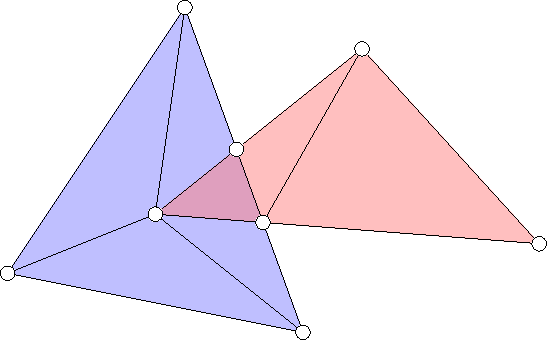
\includegraphics{\figdir/simplex-collision-resolution-2.pdf}
%   \caption{Full resolution}
% \end{figure}


% To define radial interior and radial boundary, we first define them
% for convex linear $1$-cells and then generalize.
% \begin{definition}[Radial Interior and Radial Boundary of a $1$-Cell]
%   Let $x,y \in \RR^m$ with $x \neq y$. Then the \emph{radial
%     boundary} of $C = \ip{\set{x,y}}$, denoted $\partial C$, is
%   \[
%     \partial C = \set{x,y}.
%   \]
%   We define the \emph{radial interior} of $C$ (denoted $\rint C$;
%   this is the convention given in \emph{Sakai}) to be
%   \begin{align*}
%     \rint C
%     &= C \setminus \partial C \\
%     &= \ip{\set{x,y}} \setminus \set{x,y}. \qedhere
%   \end{align*}
% \end{definition}

% \begin{definition}[Radial Interior and Radial Boundary in
%   general]\label{def:rad-int-bdy}
%   Let $C$ be a convex linear $n$-cell. Then define
%   \[
%     \rint C = \set{x \in C\MID \forall y \in C,\ \exists z \in C \st
%       x \in \rint \ip{\set{y,z}}}.
%   \]
%   Then, we have
%   \[
%     \partial C = C \setminus \rint.
%   \]
%   Note, the definition of $\rint$ is equivalent to
%   \[
%     \rint C = \set{x \in C\MID \forall y \in C,\ \exists s > 0 \st
%       [1 + s] x -  sy \in C}.\qedhere
%   \]
% \end{definition}
% % An interlude for a few important propositions:
% % \begin{leftbar}
% \begin{proposition}
%   Let $C$ be a convex linear $n$-cell. Let $\cong$ denote
%   homeomorphism. Then we have
%   \[
%     \pn{C, \partial C} \cong (B^n, S^{n-1}).
%   \]
% \end{proposition}
% \begin{sproof}
%   See \emph{Sakai}, Corollary 3.5.6 and the commentary on page
%   134.
% \end{sproof}
% \begin{proposition}
%   For any simplex $C$, $C$ has the unique topology such that $f : C
%   \times C \times I \to C$ given by
%   \[
%     f(x,y,t) = [1-t]x + ty
%   \]
%   is continuous.
% \end{proposition}
% \begin{sproof}
%   See \emph{Sakai}, Corollary 3.5.8 and the commentary on page
%   134.
% \end{sproof}
% % \end{leftbar}
% % A few more propositions before we continue.
% \begin{proposition}[Minimal Generating Set]\label{prop:min-gen-set}
%   Let $C \subset \RR^m$ be a convex linear $n$-cell. Then there
%   exists a minimal set $C^{(0)}$ such that
%   \begin{enumerate}
%     \item $\ip{C^{(0)}}  = C$, and
%     \item If $n > 0$ (i.e., $C$ is not a $0$-cell), then $C^{(0)}
%       \subset \partial C$.
%   \end{enumerate}
% \end{proposition}
% \begin{proof}
%   See \emph{Sakai}, Proposition 4.1.2 (page 136).
% \end{proof}
% \begin{definition}[Face at $x$]
%   Let $C$ be a convex linear $n$-cell, and let $x \in C$. Then the
%   \emph{face} of $C$ at $x$, denoted $C_x$, is defined by
%   \[
%     C_x = \set{y \in C \MID \exists s > 0 \st [1 + s]x - sy \in C.}
%     \qedhere
%   \]
% \end{definition}
% \begin{remark}
%   Note the similarity to \cref{def:rad-int-bdy} (Radial Interior and
%   Boundary). In particular, if $x \in \rint(C)$, then $C_x = C$.
% \end{remark}
% \begin{definition}[Face of a Cell]
%   Let $C \subset \RR^m$ be an $n$-cell, and let $D \subset \RR^m$ be
%   a $k$-cell with $k \leq n$. Then we say $D$ is a \emph{face} of
%   $C$ (denoted $D \leq C$) iff $\exists x \in C \st D = C_x$.
% \end{definition}
% % {\color{red} Are these needed?
% %   \begin{proposition}
% %     Let $C \subseteq \RR^m$ be a convex linear $n$-cell. Then $C_x$
% %     is a cell with $C_x^{(0)} = C^{(0)} = C^{(0)} \cap C_x$.
% %   \end{proposition}
% %   \begin{proposition}
% %     Maybe add proposition 4.1.6 here?
% %   \end{proposition}
% %   \begin{proposition}
% %     Let $A \subset \RR^m$ such that $A \neq \varnothing$ be
% %     arbitrary. Then $A$ is an $n$-cell iff all of the following are
% %     true:
% %     \begin{enumerate}
% %       \item $\dim \aff(C) < \infty$,
% %       \item For all $x,y \in C$ with $x \neq y$, $x + \RR_+(y - x)
% %         \not \subset C$, and {\color{red} what does this mean????}
% %       \item There exist finitely many non-constant affine
% %         functionals $f_1, \ldots, f_k : \aff(C) \to \RR$ such that
% %         \[
% %         C = \bigcap_{i=1}^k f^{-1}_i\pn{\RR_+}
% %         \]
% %     \end{enumerate}
% %   \end{proposition}
% % }

% \section{Simplicial Complexes}
% OK: from now on, we'll basically just be interested in simplicial
% complexes and their properties. The hope is that we'll be able to
% figure out which parts of Reidemeister's theorem can generalize nicely
% to wild knots.
% \begin{definition}[Cell Complex]
%   Let $I$ be an arbitrary indexing set, and let $K = \set{C_i}_{i\in
%     I}$ where each $C_i\subseteq \RR^m$ is a convex linear
%   $n_i$-cell (where $0 \leq n_i \leq m$). Then we call $K$ a
%   \emph{convex linear cell complex} iff
%   \begin{enumerate}
%     \item (\textbf{Closure under subcell}): For all $C_i \in K$, we
%       have that for all subcells $D \leq C_i$, $D \in K$ as well.
%     \item (\textbf{Closure under intersection}): For all $C_i, C_j
%       \in K$ with $C_i \cap C_j \neq \varnothing$, we have
%       \[
%       C_i \cap C_j \leq C_i \qquad\qquad\text{and}\qquad\qquad
%       C_i \cap C_j \leq C_j. \qedhere
%       \]
%   \end{enumerate}
% \end{definition}
% \begin{definition}[Simplicial Complex]
%   Let $K$ be a convex linear cell complex. We call $K$ a
%   \emph{simplicial complex} iff all of the $C_i$ are simplices.
% \end{definition}
% \begin{definition}[Polyhedron of $K$]
%   We define the \emph{polyhedron} of $K$ (denoted $\abs{K}$) by
%   \[
%     \abs{K} = \bigcup_{C \in K} \rint C \qedhere
%   \]
% \end{definition}
% \begin{definition}[Whitehead Topology]
%   Let $U \subseteq \abs{K}$. Then we say $U$ is open iff for all $C
%   \in K$, $U \cap C$ is open in $C$.
%   % \[
%   %   \ms T_{\rm whit}= \set{}
%   % \]
% \end{definition}
% \begin{proposition}
%   Let $(X, \ms T)$ be an arbitrary topological space. Then for any
%   continuous function $f : \abs{K} \to X$, $f$ is continuous iff
%   $\forall C_i \in K$, $f|C_i$ is continuous.
% \end{proposition}
% \begin{definition}[Star of a simplex]
%   Let $K$ be a simplicial complex, and let $C_i \in K$ be fixed.
%   Then we define the \emph{star} of $C$ in $K$ by
%   \[
%     \mrm{St}(C_i, K) = \set{D \MID \exists D' \in K \st C_i \leq D'
%       \text{ and } D \leq D'}. \qedhere
%   \]
% \end{definition}
% \begin{remark}
%   It's very important that we have $D \leq D'$ and not $D'\leq D$.
%   We are looking at the set of all simplices $D$ such that
%   \emph{both} $C_i$ and $D$ are faces of some larger simplex $D'$.
%   % Note, sub-faces of $D$ aaaaaaaaaAAAAAAAAAAAAAAAAAAa {\color{red}
%   %   aaaaaaaaaaaaaaaaaa}
% \end{remark}



\section{Some Examples of Rigorously-Constructing Ambient
  Isotopies}\label{sec:rigorous-ambient-isotopy}
\def\figdir{figures/infinite-gauss-sequence/}

Rigorously constructing ambient isotopies can be tedious and
unpleasant. However, given that our focus is on trying to provide
rigorous foundations for working with \emph{topological} ambient
isotopies, we'll include some notes on this process below. As with the
rest of the material in the appendix, this is strictly optional.

\begin{proposition}\label{prop:pt-to-barycenter}
  Let $\triangle_0$ be an $n$-simplex, and let $x_0 \in
  \triangle_0^\circ$ be arbitrary. Denote the barycenter of
  $\triangle_0$ by $c_0$. Then there exists an ambient isotopy
  $\ms{C}_{x_0} : [0,1] \times \RR^n \to \RR^n$ such that
  $\ms{C}_{x_0}$ is identity outside of $\triangle_0^\circ$ and
  $\ms{C}_{x_0}(1, x_0) = c_0$.
\end{proposition}
\begin{proof}
  Let $p \in \triangle_0^\circ$ be arbitrary. Then there exists a
  unique ``anchor point'' $a_p \in \partial \triangle_0$ such that
  there exists $s_p \in [0,1]$ such that $p = s_p \cdot x_0 +
  (1-s_p) \cdot a_p$. Note, this is equivalent to saying that
  $a_p, p, x_0$ are \emph{colinear} and either $p = a_p$, $p =
  x_0$, or $p$ is \emph{strictly} between $a_p$ and $x_0$. These
  lines are drawn in \emph{light orange} in
  \cref{fig:pt-to-barycenter}.


  \textbf{Claim:} Let $x(t) = t \cdot c_0 + (1-t)x_0$ (note, this
  is the straight-line homotopy from $x_0$ to $c_0$). Then the
  desired ambient isotopy $\ms C_{x_0}$ is given by
  \[
    \ms{C}_{x_0}(t, p) = s_p \cdot x(t) + (1-s_p) \cdot a_p
    \tag{$\forall p \in \triangle_0$}.
  \]
  See \cref{fig:pt-to-barycenter} for an illustration.
  \begin{figure}[H]
    \centering
    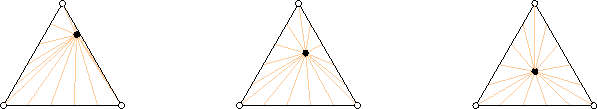
\includegraphics[scale=1]{\figdir/pt-to-barycenter.pdf}
    \caption{The desired ambient isotopy}
    \label{fig:pt-to-barycenter}
  \end{figure}
  \textbf{Proof of Claim:} First, we show (a) that the proposed
  $\ms{C}_{x_0}$ doesn't send points outside of $\triangle_0$, (b)
  that we have identity on the boundary, and (c) that we indeed
  have an ambient isotopy.
  \begin{enumerate}
    \item We want to show $\ms{C}_{x_0}$ doesn't send points outside
      of $\triangle_0$. Note, $x(t) \in \triangle_0$ for all $t$. Also
      note that $s_p + (1 - s_p) = 1$ always. Since $a_p \in
      \triangle_0$ as well, this shows $\ms{C}_{x_0}$ is a convex
      combination of points in $\triangle_0$. Since $\triangle_0$ is
      convex, it follows that $\ms{C}_{x_0}(t,p) \in \triangle$ for
      all $t \in [0,1]$, $p \in \triangle_0$. \cmark

    \item We want to show $\ms{C}_{x_0}$ is identity on the boundary.
      Note that if $p \in \partial \triangle_0$, then $p = a_p$ and
      hence $s_p = 0$. It follows that $\ms{C}_{x_0}(t, \cdot)$ is
      identity on $\partial \triangle_0$. \cmark
    \item To show that $\ms{C}_{x_0}(t, x)$ is an ambient isotopy,
      we must demonstrate that it is identity at $t=0$, that the
      image of $\triangle_0$ at $t=1$ is the desired modified
      version, that $\ms{C}_{x_0}(t, \cdot)$ is a homeomorphism for
      each $t$, and finally, that $\ms{C}_{x_0}$ is continuous
      overall.
      \begin{enumerate}[label=(\roman*)]
        \item The desired properties at $t = 0, 1$ follow
          immediately from the definition.
        \item We want to show that $\ms{C}_{x_0}(t, \cdot)$ is a
          homeomorphism for each $t$. Hence, let $t_0 \in [0,1]$ be
          arbitrary. Write $x(t_0) = x_0 + \delta(t_0)$ (from the
          definition of $x(t)$ above, we have $\delta(t_0) = t_0(c_0 -
          x_0)$). Now, note that
          \begin{align*}
            \ms{C}_{x_0}(t_0, p)
            &= s_p \cdot (x_0 + t_0(c_0 - x_0)) + (1-s_p) a_p \\
            &= \pn[Big]{s_p x_0 + (1-s_p) a_p} + s_pt_0 (c_0 - x_0) \\
            &= p + s_p t_0(c_0 - x_0).
          \end{align*}
          Ok now the $\varepsilon$-$\delta$ part: Let $\varepsilon > 0$
          be given. Through some fairly unpleasant trig, one can find a
          $\delta_0 > 0$ such that $q \in B_{\delta_0}(p)$ implies the
          angle $\angle p x_0 q$ is arbitrarily small.
          Then  one can then show that the rays
          $\overrightarrow{x_0 p}$ and $\overrightarrow{x_0 q}$
          intersect $\partial \triangle_0$ at points that are
          arbitrarily close. From this, we can constraint $\abs{s_p -
          s_q} < \varepsilon$, and use this to show continuity.

          To see that $C_{x_0}(t_0, \cdot)$ has a continuous inverse,
          observe that $p$ and $\ms{C}_{x_0}(t_0, p)$ have the same
          anchor point $a_p$ and displacement parameter $s_p$. Thus,
          define
          \[
          \ms{C}^{-1}_{x_0}(t_0, p) = s_p x(t_0) - s_p t_0 (c_0 -
          x_0),
          \]
          and note that this is indeed a well-defined inverse, and the
          same continuity argument as above demonstrates that it is
          continuous.
        \item One can then directly verify that $\ms{C}_{x_0}$ is
          continuous. \qedhere
      \end{enumerate}
  \end{enumerate}
\end{proof}
The second lemma is similar. We omit some of the details of the
proof since they are similar to that given above.
\begin{proposition} \label{prop:barycenter-exchange}
  Let $\triangle_0, \triangle_1$ be $n$-simplices that share an $n-1$
  face, and let $c_0, c_1$ be the barycenters of $\triangle_0,
  \triangle_1$ respectively. Then there exists an ambient isotopy
  $\ms{S}_{0,1} : [0,1] \times \RR^n \to \RR^n$ such that
  $\ms{S}_{0,1}$ is fixed on $\RR^n - (\triangle_0 \cup
  \triangle_1)^\circ$, and $\ms{S}_{0,1}(1, c_0) = c_1$.
\end{proposition}
\begin{proof}\renewcommand{\qed}{\hfill$\square$}
  The same proof as above works when $\triangle_0, \triangle_1$
  are regular (see \cref{fig:barycenter-isotopy}). However, when
  $\triangle_0, \triangle_1$ are \emph{not} regular, we have some
  additional things to worry about. In particular, $\triangle_0
  \cup \triangle_1$ might not be convex, so we can't just do a
  ``straight-line'' ambient isotopy.
  \begin{figure}[H]
    \centering
    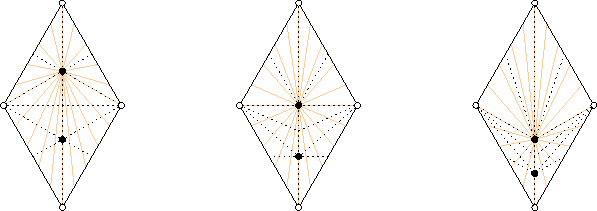
\includegraphics[scale=.8]{\figdir/barycenter-isotopy.pdf}
    \caption{The desired isotopy when the simplices are regular}
    \label{fig:barycenter-isotopy}
  \end{figure}

  If $\triangle_0 \cup \triangle_1$ is not convex, we must be a
  little more creative. In particular, we see that the ambient
  isotopy above (\cref{fig:barycenter-isotopy}) isn't actually the
  most natural choice. Instead, consider the following (see
  \cref{fig:barycenter-isotopy-nonconvex} for illustration):
  \begin{enumerate}[label=\arabic*)]\newcommand{\temd}{\text{---}\,}
    \item Let $\temd_{0,1} = \set{u_1 \cdots u_{n}}$ denote the
      shared $n-1$ face of $\triangle_0$ and $\triangle_1$. Let
      $v_0$ and $v_1$ be the vertices of $\triangle_0$ and
      $\triangle_1$ (respectively) such that $v_0, v_1 \not\in
      \temd_{0,1}$.
    \item Then note: for all $x_0 \in \triangle_0^\circ$, there
      exists a unique $y \in \temd_{0,1}$ such that $x_0$ is
      collinear with $v_0, y$. Similarly for $x_1 \in
      \triangle_1^\circ$.
    \item Now, for each $y \in \temd_{0,1}$, we join these lines
      with the following parameterization:
      \[
      Y(s) =
      \begin{cases}
        2s \cdot y\qquad\,\,\,\,\, + (1 - 2s)\cdot v_0 & s \in \bk{0, \frac{1}{2}}
        \\
        (2s - 1) \cdot v_1 + (2 - 2s)\cdot y & s \in \pb{\frac{1}{2}, 1}
      \end{cases}
      \]
      the two cases here are illustrated by the \emph{orange} and
      \emph{blue} lines in
      \cref{fig:barycenter-isotopy-nonconvex}. Note that
      $Y\pn{\frac{1}{2}} = y$. % {\color{red} How can I make the
      % notation here clearer? I feel I ought to index $Y$ by $y$.}
    \item Now we define our ambient isotopy $\ms{S}_{0,1}$. First,
      we need to look at the kinked line $Y_c(s)$ the barycenters
      of $\triangle_0, \triangle_1$ live on. The corresponding
      $s_0, s_1$ will be necessary in defining $\ms{S}_{0,1}$.


      Let's do it. Let $c_0, c_1$ be the barycenters of $\triangle_0,
      \triangle_1$ respectively. We want to show they really \emph{do}
      lie on the same $Y$. To that end, note that the line through
      $v_0, c_0$ to $\temd_{0,1}$ and the line from $v_1, c_1$ to
      $\temd_{0,1}$ both end at the barycenter of $\temd_{0,1}$ (to
      verify this, write everything in barycentric coordinates).
      Hence, the corresponding $Y$ (denote it $Y_c$) satisfies $c_0,
      c_1 \in Y_c([0,1])$. Thus there exists $s_0, s_1$ such that
      $Y_c(s_0) = c_0$, and $Y_c(s_1) = c_1$. In particular, one can
      show that $s_0 = \frac{1}{3}$, $s_1 = \frac{2}{3}$ independent
      of the choice of $\triangle_0, \triangle_1$.

      Now we can define $\ms{S}_{0,1}$ itself. To do so, we'll
      introduce a fairly complicated formula (which exposes more
      information about how we derived the formula) and then show
      that it simplifies from a complete mess to something very
      simple. Let $x \in (\triangle_0 \cup \triangle_1)^\circ$ be
      arbitrary. Write it as $Y(s_0)$ for some $Y$ as described
      above in step 3). We define $\ms{S}_{0,1}$ by
      \[
      \ms{S}_{0,1}(t, x) = \ms{S}_{0,1}(t, Y(s)) =
      \begin{cases}
        Y\pn{t\bk{s_1 - s_0 + s} + \bk{1-t}s} & s \in \bk{0,
          \frac{1}{2}} \\
        Y\pn{ \text{some mystery function!}
          % t\bk{\frac{1}{2} + ()}
        } & s \in \bk{\frac{1}{2}, 1},
      \end{cases}
      \]
      where we leave the reader to puzzle out what the mystery
      function is.
      % {\color{red} \Huge Return and finish}
  \end{enumerate}
  It follows that $\ms{S}_{0,1}$ is the desired ambient isotopy.
  \begin{figure}[H]
    \centering
    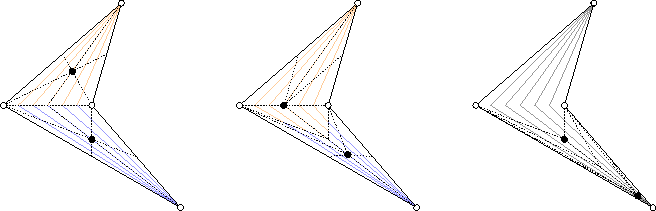
\includegraphics{\figdir/barycenter-isotopy-nonconvex-setup.pdf}
    \caption{An example where $\triangle_0 \cup \triangle_1$ is not
      convex (see \textbf{Important Note} below).}
    \label{fig:barycenter-isotopy-nonconvex}
  \end{figure}
  \textbf{Important Note:} Not all of the dotted lines are drawn in
  the final diagram, and I've removed the color-coding. I'm not
  terribly pleased with this, but it was getting to be too
  troublesome to do all of the trig arithmetic in TikZ to justify
  continuing onwards. The point is that one should imagine extending
  the reasoning of the first two diagrams, and observe that the
  barycenter gets where it needs to go.
\end{proof}

\begin{corollary}\label{cor:moving-through-simplices}
  Let $\triangle_0, \triangle_1, \ldots, \triangle_k$ be
  $n$-simplices such that for each $i = 0, \ldots, k-1$,
  $\triangle_{i}$ and $\triangle_{i+1}$ share an $n-1$-face. Let
  $x_0 \in \triangle_0$ and $x_1 \in \triangle_k$. Then there
  exists an ambient isotopy $H_{x_0, x_1} : [0,1] \times \RR^n \to
  \RR^n$ such that $H$ is fixed outside of $\bigcup_{i=0}^k
  \triangle_k^\circ$, i.e.
  \[
    H(t, x) = x \qquad\text{\rm whenever}\qquad x \in \RR^n -
    \bigcup_{i=0}^k \triangle_k^\circ,
  \]
  and $H(1, x_0) = x_1$.
\end{corollary}
\begin{proof}\renewcommand{\qed}{\hfill$\square$}
  Note, by \cref{prop:pt-to-barycenter}, there exists an ambient
  isotopy $\ms{C}_{x_0} : [0,1] \times \RR^n \to \RR^n$ that
  leaves $\RR^n - \triangle_0^\circ$ fixed, and takes $x_0$ to the
  barycenter $c_0$ of $\triangle_0$.

  Now, by \cref{prop:barycenter-exchange}, there exists a sequence
  of ambient isotopies $\ms{S}_{0,1}$, $\ms{S}_{1,2}$, $\ldots$,
  $\ms{S}_{k-1,k}$ taking the barycenter of $\triangle_0$ to that of
  $\triangle_1$, the barycenter of $\triangle_1$ to $\triangle_2$,
  and so on. For each $i \in \set{0, \ldots, k-2}$, let $f_i(x) =
  \ms S_{i,i+1}(1, x)$ It follows that $\ms S_{0,k}$ defined by
  \[
    \ms{S}_{0,k} =
    \begin{cases}
      \ms{S}_{0,1}\pn{k \cdot t, x} & t \in \bk{0, \frac{1}{k}} \\
      \ms{S}_{1,2}\pn{(k \cdot t) - 1, f_0(x)} & t \in
      \bk{\frac{1}{k}, \frac{2}{k}} \\
      \vdots & \\
      \ms{S}_{i,i+1}\pn{(k \cdot t) - i, \comp_{j=1}^{i-1} f_j(x)} &
      t \in \bk{\frac{i}{k}, \frac{i+1}{k}} \\
      \vdots & \\
      \ms{S}_{k-1,k}\pn{(k \cdot t) - (k-1), \comp_{j=1}^{k-2}
        f_j(x)} & t \in
      \bk{\frac{k-1}{k}, 1} \\
    \end{cases}
  \]
  can be shown to be a valid ambient isotopy.\footnote{Just apply
    the gluing lemma.}
\end{proof}
% \begin{figure}[H]
%   \centering
%   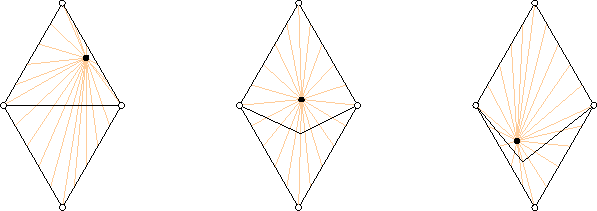
\includegraphics{\figdir/two-simplex-isotopy.pdf}
%   \caption{One way to deform the space to get $x_0 \to x_1$.}
% \end{figure}

  % \begin{lemma}
  %   Suppose $f : \RR^3 \to \RR^3$ is an orientation-preserving
  %   homeomorphism with $f(K) = P$. Then there exists an ambient
  %   isotopy $H : [0,1] \times \RR^n \to \RR^n$ such that $H(1, f)$
  %   fixes a 3-simplex.
  % \end{lemma}
  % \emph{Proof:} We construct the vertices of our simplex $[v_0 v_1
  % v_2 v_3]$. We have cases:
  % \begin{enumerate}[label=(\arabic*)]
  %   \item Suppose $f$ has a fixed point. Then let this be $v_0$.
  %   \item Else, we want to show there exists an ambient isotopy $H^0
  %     : [0,1] \times \RR^3 \to \RR^3$ such that $H^0(1, f(v_0)) =
  %     v_0$. We'll {\color{red} this part currently unfinished}
  %     % let $S \subseteq \RR^3$ be an arbitrary 3-simplex,
  %     % and let $v_0$ .
  %   \item Then consider the ambient isotopy $G : [0,1] \to \RR^3$
  %     that leaves $\RR^3 \setminus S$ fixed (only deforms the interior
  %     of $S$). {\color{red} Also unfinished}
  % \end{enumerate}

  % % \begin{lemma}
  % %   Let $\triangle_1, \triangle_2, \ldots, \triangle_n$ be a sequence of
  % %   $3$-simplices such that for each $k = 1,\ldots, n-1$, the
  % %   simplices $\triangle_{k}$ and $\triangle_{k+1}$ share a common
  % %   $2$-face. Now, let $x_0 \in \triangle_1$ and $x_1 \in \triangle_n$.
  % %   Then there exists an ambient isotopy $H : [0,1] \to \RR^3$ such
  % %   that $H$ is fixed outside the simplices, i.e.
  % %   \[
  % %     H(t, x) = x \qquad \text{\rm whenever } \qquad x \in \RR^3 -
  % %     \bigcup_{k=1}^n \triangle_k,
  % %   \]
  % %   and we have
  % %   \[
  % %     H(1, x_0) = x_1.
  % %   \]
  % % \end{lemma}
  % % \emph{Proof:}





% \begin{leftbar}
%   \begin{lemma}
%     Let all variables as quantified above, except choosing $K$
%     restricted to a connected subset of $S^1$ (think of this as
%     embedding an interval). \textbf{Further} suppose that $K$ is
%     wild at exactly one point $p$. Then the claim holds.
%   \end{lemma}
%   \emph{Proof of Lemma:} Let $\pn{V_k}_{k=0}^\infty$ be a nested
%   sequence of closed neighborhoods of $p$. Explicitly: each $V_k$ is
%   closed, and
%   \[
%     \bigcap_{k=0}^\infty V_k = \set{p} \qquad\qquad\qquad \text{and}
%     \qquad\qquad\qquad
%     \cdots \subseteq V_2 \subseteq V_1 \subseteq V_0.
%   \]
%   Since $K$ is ambient isotopic to a polygonal knot, there exists an
%   orientation-preserving homeomorphism $h : \RR^3 \to \RR^3$ such
%   that $h(K) = P$. Note, it follows that
%   \[
%     \bigcap_{k=0}^\infty h(V_k) = \set{h(p)} \qquad\qquad\qquad
%     \text{and} \qquad\qquad\cdots \subseteq h(V_2) \subseteq h(V_1)
%     \subseteq h(V_0).
%   \]
%   Since $P$ has only finitely many crossings, it follows that there
%   exists $N \in \NN$ such that for $n > N$, $P$ contains no
%   crossings in $h(V_n)$. Equivalently, $h(V_n) - P = h(V_n) - h(K) =
%   h(V_n - K)$ has trivial fundamental group.

%   {\color{red} this is unfinished}

%   \textbf{Claim:} There exists an ambient isotopy $f : \RR^3 \to
%   \RR^3$ such that $f(1, h(V_n)) = h(V_n)$ for all $n > N$.
% \end{leftbar}



%%% Local Variables:
%%% TeX-master: "../../kobayashi-thesis"
%%% End:
